\documentclass[USenglish, a4paper]{article}

\usepackage{babel}
\usepackage{graphicx,epstopdf}

\author{Tor Aksel N. Heirung}
\title{A few comments on EPS figures in MATLAB}
\date{\today}

\begin{document}

\maketitle
\thispagestyle{empty}

This note gives an example on a simple figure that looks fairly good. See the attached MATLAB code for how the figure is produced. Note that the package \emph{epstopdf} is needed to convert the figure from EPS to PDF automatically in Latex.

The result in shown in Figure~\ref{fig:testfig}. Note that the data shown is not meant to make sense. If you plot a long data vector (many elements), try to avoid using line styles such as \verb|'-o'| and \verb|'-x'| in MATLAB. Remember that it does not work very well to use colors for distinguishing graphs if you print the report in black and white.

\begin{figure}[htb]
	\centering
		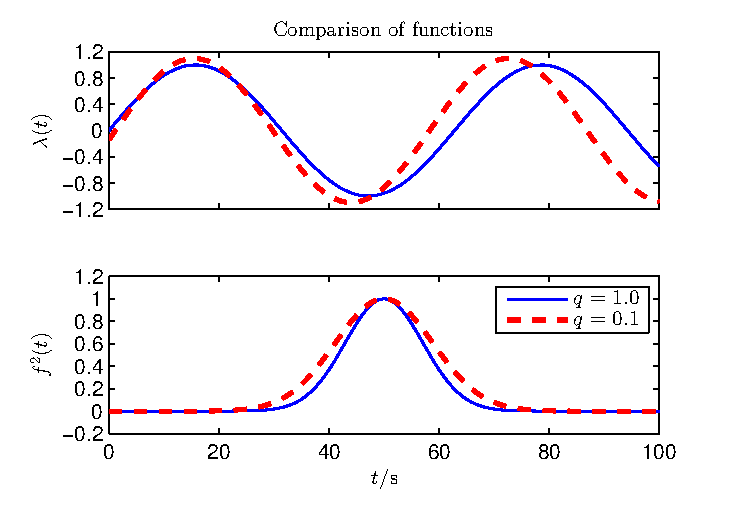
\includegraphics{testfig.eps}
	\caption{An example figure saved as EPS in MATLAB.}
	\label{fig:testfig}
\end{figure}

Since we set the width of the figure in MATLAB before we print it, it in not necessary to scale it to fit the page margins. This gives consistent font size across all figures in your report.

\end{document}